\chapter{Despliegue}
En este capítulo se analizará el despliegue de la aplicación y la manera en la que se puede realizar de manera teórica.

\section{Web Server Gateway Interface}
Django ya cuenta con una capa \emph{\gls{middleware}} que permite el uso de un \gls{WSGI} y por defecto el fichero \emph{wsgi.py} ya contiene lo necesario para utilizar un \gls{WSGI}, simplemente se tiene que lanzar el comando del gestor de tareas para que Gunicorn comience a escuchar peticiones \gls{http}. 
\begin{figure}[H!]
    \begin{lstlisting}[style=C, caption={Métodos de la base de datos utilizados para buscar recetas por ingredientes}]
        invoke runserver
    \end{lstlisting}
        \caption{Comando para lanzar Gunicorn}
        \label{cmd:gunicorn}
    \end{figure}

Gunicorn se puede ejecutar de manera manual cada vez que se reinicie el servidor, pero se recomienda encarecidamente crear un servicio utilizando el \emph{\gls{daemon} Systemd}, para ello es necesario crear un fichero con extensión \emph{.service} y habilitarlo para que se ejecute automáticamente en el arranque de sistema.

\section{Servidor Web}
La configuración básica de Nginx es muy sencilla. Siendo necesario instalar el paquete y cambiar el fichero de configuración \textit{default} en la ruta \textit{/etc/nginx/sites-available/default}, es completamente necesario cambiar la ruta de archivos estáticos y llevársela a Nginx, cambiando el parámetro \textit{STATIC\_URL} del fichero de ajustes de \gls{django}. 

Adicionalmente se necesita un host, donde alojar el servidor web, que se elegirá \textit{dietplanner.com} como dominio de prueba en el campo teórico, sin poder registrar el nombre en algún sitio de para el registro de dominios como \href{https://www.godaddy.com/es-es}{GoDaddy}.

Para aplicar el cambio de dominio, se debe cambiar el \textit{server\_name} de Nginx y el parámetro \textit{Allowed hosts} de Django, con esta información.

Se utilizará Nginx como reverse proxy para añadir más seguridad a la infraestructura del proyecto.

\section{Infraestructura en la nube}
Como servicio de infraestructura en la nube se utilizará \gls{AWS}, aunque existen otros \gls{IaaS} como Azure y Google Cloud. Pero \gls{AWS} ofrece un gran abanico de servicios que pueden ser útiles en el desarrollo del proyecto, no solo en seguridad, sino en escalabilidad. 

Para el despliegue del proyecto se pueden seguir varias alternativas, la más razonable es utilizar una instancia basada en Linux. En \gls{AWS}, las instancias se conocen como Elastic Cloud Computing (\gls{EC2}) y tienen diferentes tamaños dependiendo de que componentes se quieran potenciar. Para el proyecto se utilizarán \gls{EC2} de la familia \textit{T3}, orientada a un propósito general, en cuanto al tamaño no se esperan inicialmente demasiadas peticiones simultáneas así que se puede utilizar una instancia \textit{t3.medium} con 2vCPU y 4GB de memoria. De manera normal se utilizarán dos instancias \gls{EC2}, pero se incluye una plantilla para escalar la instancia y ejecutar la aplicación, dándose a conocer al balanceador de carga para añadir escalabilidad a la aplicación. Cuando no haya mucha carga se escalaran hacia abajo automáticamente, ahorrando costes.

Actualmente se tiene SQLite en un fichero ubicado en la raíz del proyecto, pero para añadir escalabilidad, se utilizará una instancia del servicio de base de datos relacional (\gls{RDS}) de \gls{AWS}. Actualmente no se permite el uso de SQLite en \gls{AWS}, con lo cual existen dos alternativas, confiar en SQLite3 ya que permite la lectura simultánea y no se realizará ninguna escritura o bien migrar la base de datos a una Aurora con el motor MySQL o PostgreSQL, que son menos costosas que utilizar una base de datos ``pura''. Al igual que ocurría con las \gls{EC2}, se debe elegir el tipo de instancia para la base de datos, se elegirá la más pequeña, una Aurora equilibrada. Para una alta disponibilidad de los datos, se migrarán a una Aurora, ya que la migración no incurre mucho esfuerzo, simplemente se cambia la dirección de la base de datos y se cargan los datos a la nueva \gls{RDS}, El \textit{\gls{ORM}} de \Gls{django} se encargará del resto.

Se han definido tanto la base de datos como el tipo de instancia \gls{EC2} que se utilizará, pero no existe una infraestructura de red. Para contener la infraestructura en la nube de manera privada, se utiliza una \textit{Virtual Private Cloud} a la que se le asigna un bloque \textit{\gls{CIDR}}, permitiendo que la infraestructura interna cuente con una dirección privada para cada recurso. La red de una VPC se subdivide en \textit{subnets}, partiendo ese bloque \textit{\gls{CIDR}} en pequeñas redes orientadas al uso por parte de diferentes servicios. Para este proyecto solo serán necesarias una \textit{subnet} para la \gls{EC2} y dos \textit{subnets} para una \gls{RDS} con alta disponibilidad, dividiéndose en varias zonas de disponibilidad de Amazon. 

En cuestión de seguridad, las \textit{subnet} cuentan con una \textit{Access Control List} (\gls{ACL}) que por defecto deja pasar cualquier tráfico en la red, para proteger las instancias normalmente se utilizan grupos de seguridad con reglas explícitas. Por ejemplo, se debe poder permitir la gestión de una instancia a través de \gls{SSH} solo para determinado grupo de personas. Para ello se puede utilizar un \textit{site-to-site-VPN} ofrecido por Amazon, que conecta el equipo local con las instancias a través de un túnel \gls{VPN}. Y configurar el grupo de seguridad para permitir solo las conexiones \gls{SSH} a esa instancia. De la misma manera será necesario crear un grupo de seguridad para las conexiones a través del puerto 5432 para PostgreSQL o del puerto 3306 para MySQL.

Para permitir el acceso a la aplicación de manera segura, se utilizará un \emph{Elastic Load Balancer} (\gls{ELB}) que actúe como una capa de seguridad, transportando únicamente las peticiones \glspl{http} a la instancia \gls{EC2} con nuestra aplicación, sin abrir dicha instancia a internet. El balanceador de carga, desechará toda petición que no sea \gls{http}, las conexiones no seguras en el puerto 80 se pueden redirigir al puerto 443, pero para ello es necesario un certificado. Amazon ofrece su propio servicio de certificados, solo aplicables al entorno de \gls{AWS}, pero por ahora es suficiente. Este balanceador tiene una dirección pública que se registrará como dominio, al resolver el dominio en un servidor \gls{DNS}, se obtendrá esta dirección pública. 

Para conectar la instancia a internet y ser capaces de descargar actualizaciones es necesarias de seguridad y mantenimiento es necesario una \textit{Internet Gateway}, que tiene su coste a parte. 

En conclusión, la infraestructura descrita quedaría así:
\begin{figure}[H]
    \fbox{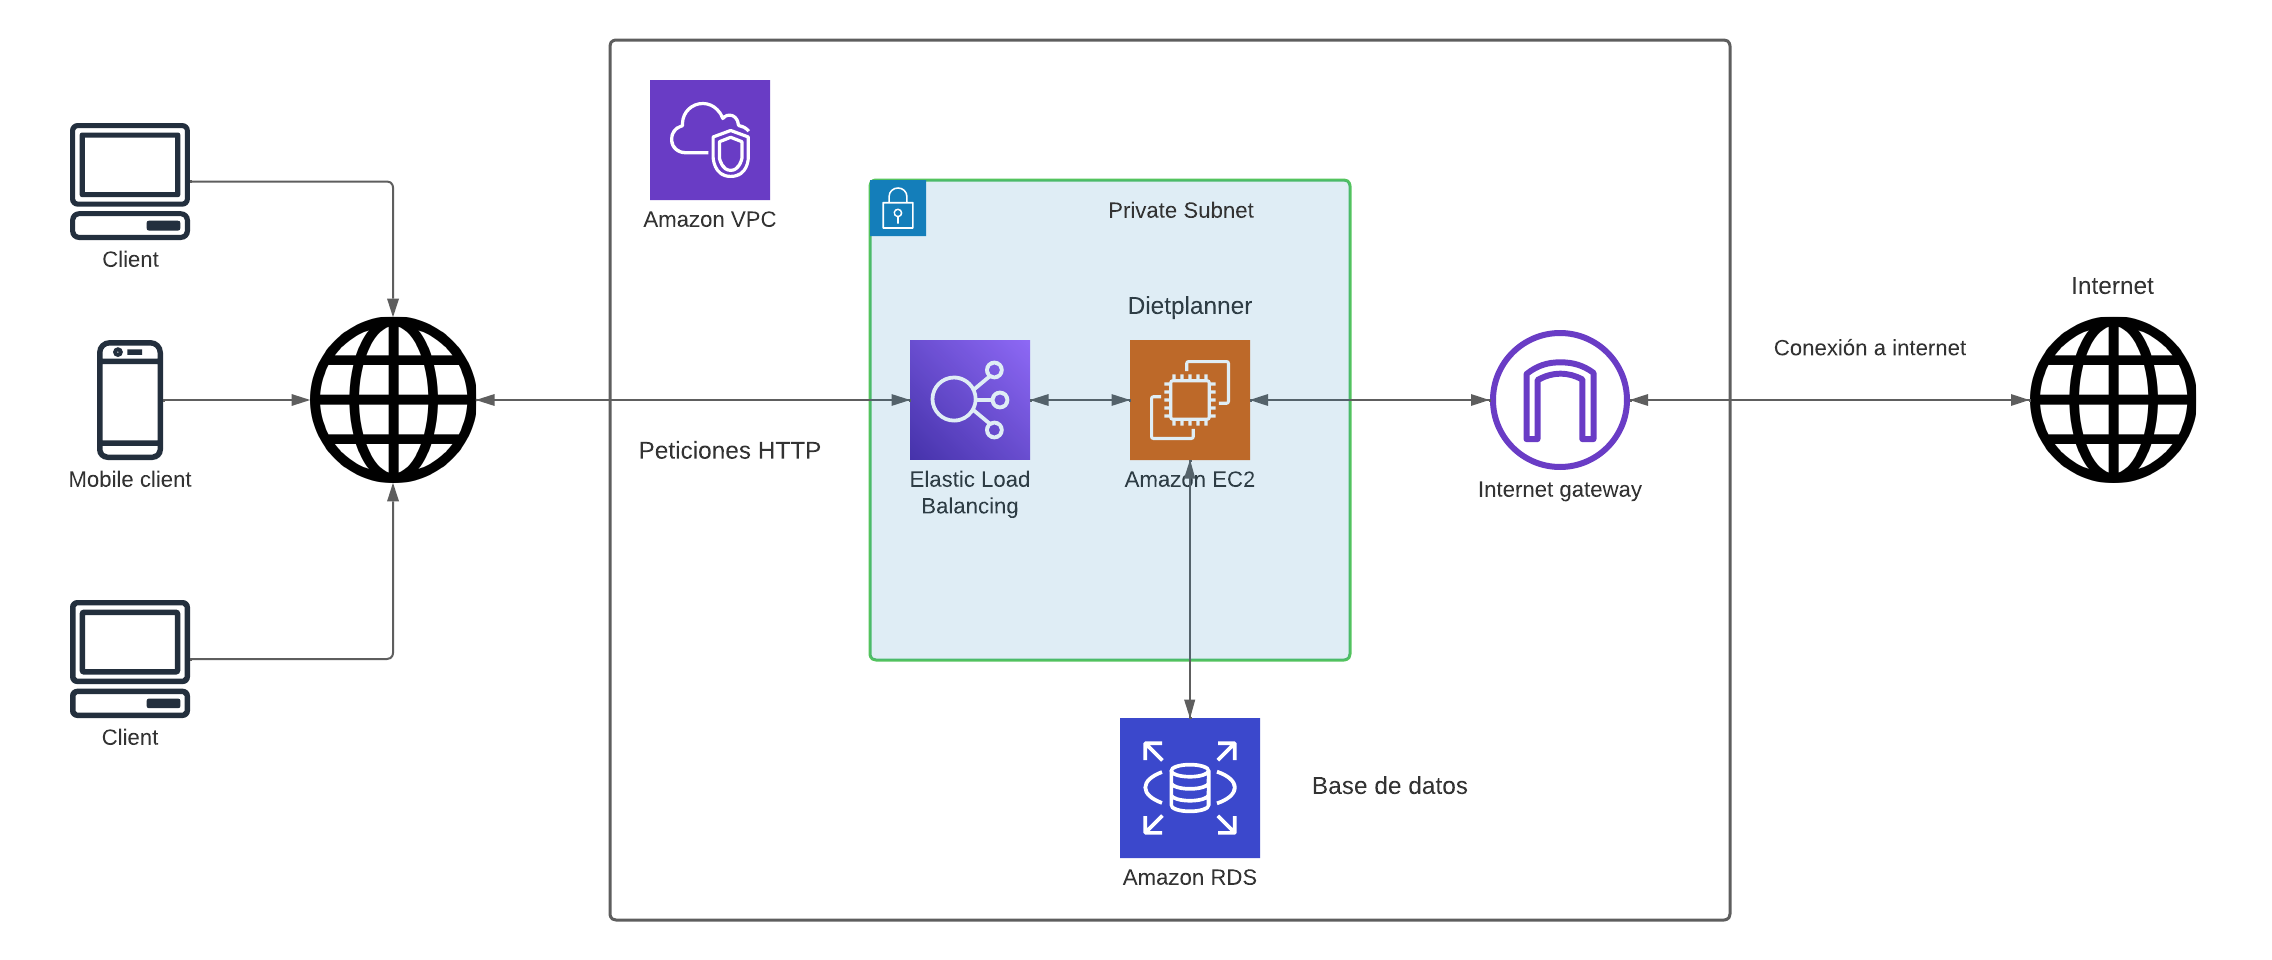
\includegraphics[width=125mm, scale=1]{./doc/imagenes/infra.png}}
    \caption{Diagrama de infraestructura}
    \label{fig:infra}
\end{figure}